% Options for packages loaded elsewhere
% Options for packages loaded elsewhere
\PassOptionsToPackage{unicode}{hyperref}
\PassOptionsToPackage{hyphens}{url}
%
\documentclass[
  ignorenonframetext,
  aspectratio=169,
  handout]{beamer}
\newif\ifbibliography
\usepackage{pgfpages}
\setbeamertemplate{caption}[numbered]
\setbeamertemplate{caption label separator}{: }
\setbeamercolor{caption name}{fg=normal text.fg}
\beamertemplatenavigationsymbolsempty
% remove section numbering
\setbeamertemplate{part page}{
  \centering
  \begin{beamercolorbox}[sep=16pt,center]{part title}
    \usebeamerfont{part title}\insertpart\par
  \end{beamercolorbox}
}
\setbeamertemplate{section page}{
  \centering
  \begin{beamercolorbox}[sep=12pt,center]{section title}
    \usebeamerfont{section title}\insertsection\par
  \end{beamercolorbox}
}
\setbeamertemplate{subsection page}{
  \centering
  \begin{beamercolorbox}[sep=8pt,center]{subsection title}
    \usebeamerfont{subsection title}\insertsubsection\par
  \end{beamercolorbox}
}
% Prevent slide breaks in the middle of a paragraph
\widowpenalties 1 10000
\raggedbottom
\AtBeginPart{
  \frame{\partpage}
}
\AtBeginSection{
  \ifbibliography
  \else
    \frame{\sectionpage}
  \fi
}
\AtBeginSubsection{
  \frame{\subsectionpage}
}
\usepackage{iftex}
\ifPDFTeX
  \usepackage[T1]{fontenc}
  \usepackage[utf8]{inputenc}
  \usepackage{textcomp} % provide euro and other symbols
\else % if luatex or xetex
  \usepackage{unicode-math} % this also loads fontspec
  \defaultfontfeatures{Scale=MatchLowercase}
  \defaultfontfeatures[\rmfamily]{Ligatures=TeX,Scale=1}
\fi
\usepackage{lmodern}

\ifPDFTeX\else
  % xetex/luatex font selection
\fi
% Use upquote if available, for straight quotes in verbatim environments
\IfFileExists{upquote.sty}{\usepackage{upquote}}{}
\IfFileExists{microtype.sty}{% use microtype if available
  \usepackage[]{microtype}
  \UseMicrotypeSet[protrusion]{basicmath} % disable protrusion for tt fonts
}{}
\makeatletter
\@ifundefined{KOMAClassName}{% if non-KOMA class
  \IfFileExists{parskip.sty}{%
    \usepackage{parskip}
  }{% else
    \setlength{\parindent}{0pt}
    \setlength{\parskip}{6pt plus 2pt minus 1pt}}
}{% if KOMA class
  \KOMAoptions{parskip=half}}
\makeatother


\usepackage{longtable,booktabs,array}
\newcounter{none} % for unnumbered tables
\usepackage{calc} % for calculating minipage widths
\usepackage{caption}
% Make caption package work with longtable
\makeatletter
\def\fnum@table{\tablename~\thetable}
\makeatother
\usepackage{graphicx}
\makeatletter
\newsavebox\pandoc@box
\newcommand*\pandocbounded[1]{% scales image to fit in text height/width
  \sbox\pandoc@box{#1}%
  \Gscale@div\@tempa{\textheight}{\dimexpr\ht\pandoc@box+\dp\pandoc@box\relax}%
  \Gscale@div\@tempb{\linewidth}{\wd\pandoc@box}%
  \ifdim\@tempb\p@<\@tempa\p@\let\@tempa\@tempb\fi% select the smaller of both
  \ifdim\@tempa\p@<\p@\scalebox{\@tempa}{\usebox\pandoc@box}%
  \else\usebox{\pandoc@box}%
  \fi%
}
% Set default figure placement to htbp
\def\fps@figure{htbp}
\makeatother





\setlength{\emergencystretch}{3em} % prevent overfull lines

\providecommand{\tightlist}{%
  \setlength{\itemsep}{0pt}\setlength{\parskip}{0pt}}



 


\makeatletter
\@ifpackageloaded{caption}{}{\usepackage{caption}}
\AtBeginDocument{%
\ifdefined\contentsname
  \renewcommand*\contentsname{Table of contents}
\else
  \newcommand\contentsname{Table of contents}
\fi
\ifdefined\listfigurename
  \renewcommand*\listfigurename{List of Figures}
\else
  \newcommand\listfigurename{List of Figures}
\fi
\ifdefined\listtablename
  \renewcommand*\listtablename{List of Tables}
\else
  \newcommand\listtablename{List of Tables}
\fi
\ifdefined\figurename
  \renewcommand*\figurename{Figure}
\else
  \newcommand\figurename{Figure}
\fi
\ifdefined\tablename
  \renewcommand*\tablename{Table}
\else
  \newcommand\tablename{Table}
\fi
}
\@ifpackageloaded{float}{}{\usepackage{float}}
\floatstyle{ruled}
\@ifundefined{c@chapter}{\newfloat{codelisting}{h}{lop}}{\newfloat{codelisting}{h}{lop}[chapter]}
\floatname{codelisting}{Listing}
\newcommand*\listoflistings{\listof{codelisting}{List of Listings}}
\makeatother
\makeatletter
\makeatother
\makeatletter
\@ifpackageloaded{caption}{}{\usepackage{caption}}
\@ifpackageloaded{subcaption}{}{\usepackage{subcaption}}
\makeatother

\usepackage{bookmark}
\IfFileExists{xurl.sty}{\usepackage{xurl}}{} % add URL line breaks if available
\urlstyle{same}
\hypersetup{
  pdftitle={The Need for Quantization},
  pdfauthor={Davit Potoyan},
  hidelinks,
  pdfcreator={LaTeX via pandoc}}


\title{\texorpdfstring{The Need for
Quantization}{The Need for Quantization}}
\subtitle{\texorpdfstring{Chem 3240 · Lecture
1.2}{Chem 3240 · Lecture 1.2}}
\author{Davit Potoyan}
\date{}

\begin{document}
\frame{\titlepage}


\begin{frame}
\begin{block}{What is the nature of light?}
\protect\phantomsection\label{what-is-the-nature-of-light}
\begin{columns}[T]
\begin{column}{0.5\linewidth}
\includegraphics[width=0.9\linewidth,height=\textheight,keepaspectratio]{../../ch01/images/EM-Wave.gif}
\end{column}

\begin{column}{0.5\linewidth}
\begin{itemize}
\tightlist
\item
  Light as a \textbf{traveling electromagnetic wave}
\item
  Perpendicular \textbf{electric} and \textbf{magnetic} components
\item
  Needs \textbf{no medium}, travels in vacuum at speed \(c\)
\item
  This wave picture is \textbf{not the whole story}
\end{itemize}
\end{column}
\end{columns}
\end{block}

\begin{block}{The electromagnetic spectrum}
\protect\phantomsection\label{the-electromagnetic-spectrum}
\begin{columns}[T]
\begin{column}{0.55\linewidth}
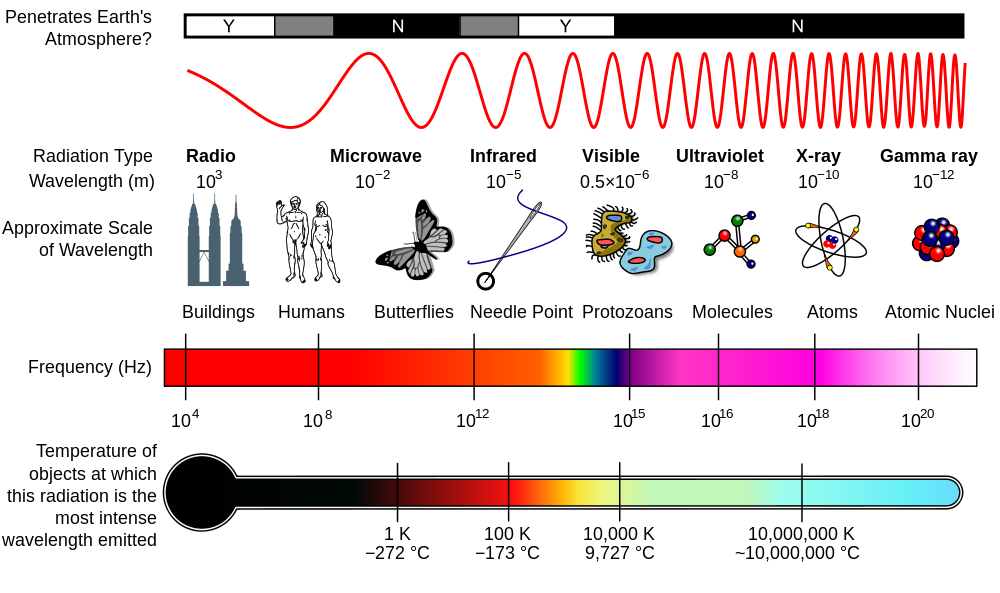
\includegraphics[width=0.95\linewidth,height=\textheight,keepaspectratio]{../../ch01/images/lec1_EMspec.jpg}
\end{column}

\begin{column}{0.45\linewidth}
\begin{itemize}
\tightlist
\item
  \textbf{Visible light} is a narrow band
\item
  \textbf{High frequency} carries \textbf{more energy} (X-rays, gamma)
\item
  \textbf{Low frequency} carries \textbf{less energy} (microwave, radio)
\item
  Clear link between an object's \textbf{temperature} and its radiation
\end{itemize}
\end{column}
\end{columns}
\end{block}

\begin{block}{Frequency, wavelength, speed of light}
\protect\phantomsection\label{frequency-wavelength-speed-of-light}
\[\lambda \nu = c\]

\begin{itemize}
\tightlist
\item
  \textbf{Speed of light}: \(c = 3 \cdot 10^8 \, m/s\) (fundamental
  constant)
\end{itemize}

\begin{itemize}
\tightlist
\item
  \textbf{Frequency} \(\nu\): cycles per second, \(1\,Hz = 1\,s^{-1}\)
\end{itemize}

\begin{itemize}
\tightlist
\item
  \textbf{Wavelength} \(\lambda\): distance between successive peaks
\end{itemize}

\begin{itemize}
\tightlist
\item
  Key question: how does \textbf{energy} \(E\) relate to
  \textbf{frequency} \(\nu\)?
\end{itemize}
\end{block}

\begin{block}{The black body}
\protect\phantomsection\label{the-black-body}
\begin{columns}[T]
\begin{column}{0.45\linewidth}
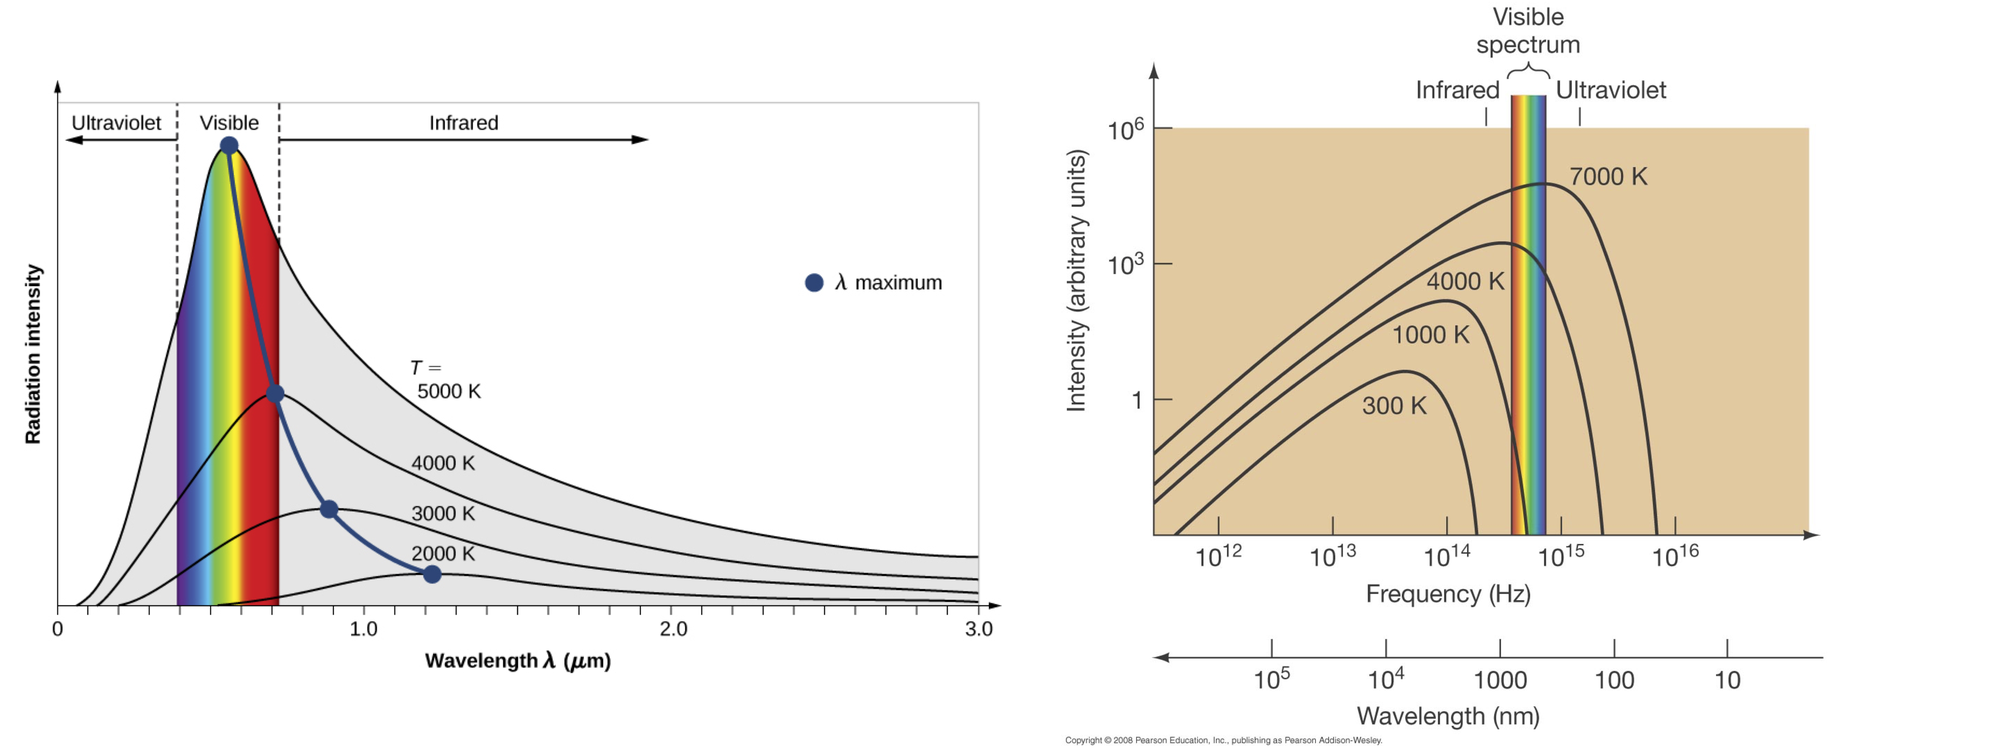
\includegraphics[width=0.95\linewidth,height=\textheight,keepaspectratio]{../../ch01/images/lec1_bb.png}
\end{column}

\begin{column}{0.55\linewidth}
\begin{itemize}
\tightlist
\item
  \textbf{Idealized model}: absorbs and emits \textbf{every wavelength}
\item
  In thermal equilibrium at temperature \(T\)
\item
  Emitted spectrum set \textbf{only by} \(T\)
\item
  Heating up: (1) \textbf{intensity rises}, (2) peak \textbf{shifts to
  higher} \(\nu\), (3) color \textbf{red to yellow to blue}
\end{itemize}
\end{column}
\end{columns}
\end{block}

\begin{block}{The classical picture}
\protect\phantomsection\label{the-classical-picture}
\begin{columns}[T]
\begin{column}{0.45\linewidth}
\includegraphics[width=0.95\linewidth,height=\textheight,keepaspectratio]{../../ch01/images/phonons.gif}
\end{column}

\begin{column}{0.55\linewidth}
\begin{itemize}
\tightlist
\item
  Heated atoms vibrate like \textbf{springs}, radiating at frequency
  \(\nu\)
\item
  More \textbf{short-wavelength} modes fit in a box than long ones:
  \[dN_{\nu} = \frac{8\pi}{c^3} \cdot \nu^2 d\nu\]
\item
  \textbf{Equipartition}: each oscillator gets the same energy
  \[\langle E\rangle = k_BT\]
\end{itemize}
\end{column}
\end{columns}
\end{block}

\begin{block}{The ultraviolet catastrophe}
\protect\phantomsection\label{the-ultraviolet-catastrophe}
\begin{columns}[T]
\begin{column}{0.5\linewidth}
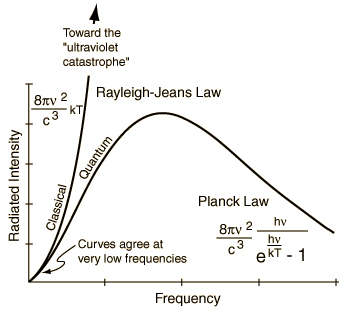
\includegraphics[width=0.9\linewidth,height=\textheight,keepaspectratio]{../../ch01/images/lec1_UVcat.jpg}
\end{column}

\begin{column}{0.5\linewidth}
\begin{itemize}
\tightlist
\item
  Classical radiation distribution:
  \[\rho({\nu}) = k_B T \cdot \frac{8\pi}{c^3}\nu^2\]
\item
  \textbf{Shoots to infinity} at high \(\nu\)
\item
  Total radiation would be \textbf{infinite}: a light bulb could destroy
  the universe
\item
  \textbf{Classical physics fails}
\end{itemize}
\end{column}
\end{columns}
\end{block}

\begin{block}{Planck's trick: quantization}
\protect\phantomsection\label{plancks-trick-quantization}
In 1900 Planck postulated that only \textbf{discrete} energy values are
allowed:

\[\boxed{E= h\nu}\]

\begin{itemize}
\tightlist
\item
  Planck's constant:
  \(h = 6.63 \cdot 10^{-34} \, \text{J} \cdot \text{s}\)
\end{itemize}

\begin{itemize}
\tightlist
\item
  Atoms absorb and emit radiation in \textbf{quanta}, multiples of
  \(h\nu\)
\end{itemize}

\begin{itemize}
\tightlist
\item
  \(h\) is tiny, so quantization is \textbf{invisible} at the macro
  scale (classical limit \(h \to 0\))
\end{itemize}
\end{block}

\begin{block}{Planck's radiation law}
\protect\phantomsection\label{plancks-radiation-law}
Quantized oscillators give a \textbf{frequency-dependent} average
energy: \[\langle E \rangle = \frac{h\nu}{e^{\frac{h\nu}{ kT}} - 1}\]

This yields a distribution that \textbf{vanishes} at high frequency:
\[\rho_{\nu}(T) = \frac{8\pi \nu^2}{c^3} \cdot \frac{1}{e^{\frac{h\nu}{kT}} - 1}\]

\begin{itemize}
\tightlist
\item
  Integrating over all \(\nu\) gives a \textbf{finite} total:
  \(\int^{\infty}_0 \rho_{\nu}(T)d\nu = \sigma T^4\)
\item
  No more catastrophe!
\end{itemize}
\end{block}

\begin{block}{Wien's displacement law}
\protect\phantomsection\label{wiens-displacement-law}
\begin{columns}[T]
\begin{column}{0.45\linewidth}
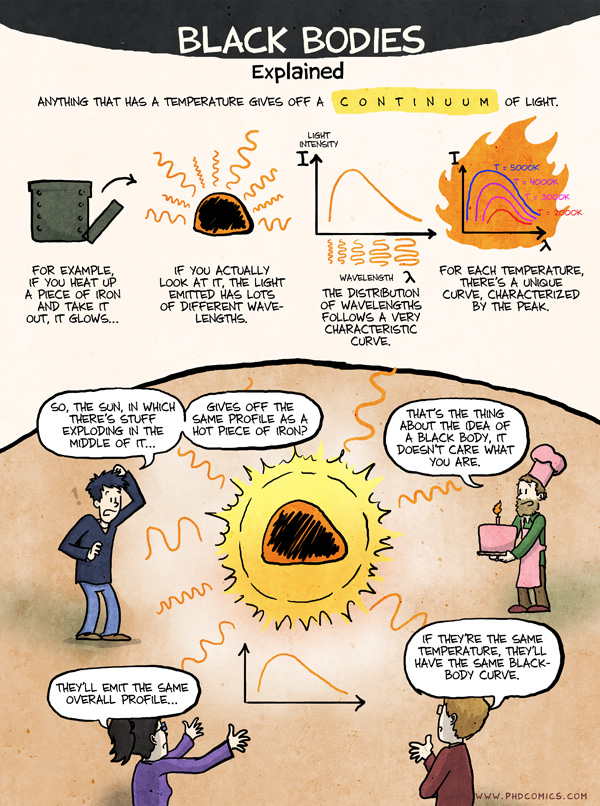
\includegraphics[width=0.95\linewidth,height=\textheight,keepaspectratio]{../../ch01/images/Black_body_rad.jpg}
\end{column}

\begin{column}{0.55\linewidth}
\begin{itemize}
\tightlist
\item
  Peak wavelength is \textbf{inversely proportional} to temperature:
  \[\lambda_{max} = \frac{b}{T}\]
\item
  \(b = 2.898 \cdot 10^{-3} \, m \cdot K\)
\item
  Connects an object's \textbf{temperature} to its \textbf{color}
\item
  Hotter object: \textbf{shorter} \(\lambda_{max}\) (bluer)
\end{itemize}
\end{column}
\end{columns}
\end{block}
\end{frame}

\begin{frame}{Takeaway}
\protect\phantomsection\label{takeaway}
\begin{quote}
Energy is \textbf{quantized}: by postulating \(E = h\nu\), Planck cured
the ultraviolet catastrophe and gave birth to quantum mechanics.
\end{quote}
\end{frame}




\end{document}
